\section{Experiments}
\label{sec:empirical_results}


\noindent\textbf{Model Architecture.}
For model architectures, we experiment with Transformer$_\text{small}$ and Transformer$_\text{base}$, following the same setting as in~\citet{Ott:2018scaling}: 6 encoder layers and 6 decoder layers on IWSLT14 and WMT14. 
We also vary the depth and width of the Transformer model on machine translation tasks. 
On IWSLT14, we use 3 different random seeds and plot the mean accuracy $\pm$ one standard deviation. 
All the embedding layers (including the final output projection layer) are also randomized and pruned unless otherwise specified. 
Moreover, on all figures, the ``fully-weighted model'' denotes the standard full model (all weights remaining). 

\noindent\textbf{Machine Translation results.}
In~\fref{fig:mt_base}, we present results for directly pruning a randomly weighted Transformer on IWSLT14 and WMT14 tasks. 
Specifically, we vary the ratio of remaining parameters in the randomized model.

As can be seen, there is no significant performance difference between a one-layer random Transformer versus a 6-layer standard random Transformer across different percents of remaining weights on IWSLT14 and WMT14. 
We also observe that having the remaining randomized weight percents approach 0 or 100 leads to the worst performance across the settings. 
This is expected since the outputs will be random when we have 100\% randomized weights, and the model will not perform well when only limited weights are unpruned (close to 0\%). 
The best performing subnetwork of a one-layer randomized Transformer has 50\% weights remained. 
Connected to the search space of the employed method where we are choosing $\sigma$\% out of 100\% randomized weights, $\sigma=50$ leads to the largest search space. 



\noindent\textbf{Effectiveness of Pre-trained Embeddding layers.}
Embedding layers are critical since they can be viewed as the inputs for an NLP model, which are analogous to the image pixels in vision. 
Plenty of prior studies have explored how to obtain the pre-trained embedding in an un-supervised way~\citep{mikolov2013efficient,pennington-etal-2014-glove}. 
We experiment with this practical setting where we could have access to the encoder/decoder embedding layers, which are pre-trained from the public checkpoint in fairseq\footnote{\href{https://github.com/pytorch/fairseq/}{https://github.com/pytorch/fairseq/}}, and we present the results in ~\fref{fig:mt_embed}. 
We observe a significant performance boost for a one-layer randomized transformer across different remaining weights. 
The difference is much larger for the bigger WMT14 dataset (around +3.0 BLEU for WMT14 and +1.0 BLEU for IWSLT14). 
The best one-layer randomized Transformer reaches 89\%/74\% of the fully-weighted Transformer performance on IWSLT14/WMT14, respectively.  


\begin{table}[]\resizebox{\linewidth}{!}{
% \small
\setlength\tabcolsep{1.5pt}
\begin{tabular}{c|ccccc}
\hline
\multicolumn{1}{c|}{Task} & Model & BLEU & \multicolumn{1}{c}{Memory} & \begin{tabular}[c]{@{}c@{}}Remaining \\ Param Ratio\end{tabular} & \begin{tabular}[c]{@{}c@{}}Param \\ (no mask)\end{tabular} \\\hline \midrule

\multirow{7}{*}{IWSLT} & Trans$_\text{small}$ & 34.66 ($\pm$0.11) & 148MB & 100.0 & 39M \\
\cline{2-6}

 & \begin{tabular}[c]{@{}c@{}}One-layer \\ Random Trans$_\text{small}$\end{tabular} & 30.95 ($\pm$0.12) & 28MB & 50.0 & 7M \\   \cline{2-6}
 & \begin{tabular}[c]{@{}c@{}}One-layer \\ Trans$_\text{wide}$\end{tabular} & 34.14 ($\pm$0.08) & 71MB & 50.0 & 18M \\\cline{2-6}
 & \begin{tabular}[c]{@{}c@{}}One-layer \\ Random Trans$_\text{deep}$\end{tabular} & 31.51 ($\pm$0.10) & 29MB & 50.0 & 7M \\\hline\midrule
\multirow{7}{*}{WMT} & Trans-base & 27.51 & 328MB & 100.0 & 86M \\\cline{2-6}
 & \begin{tabular}[c]{@{}c@{}}One-layer \\ Random Trans$_\text{base}$\end{tabular} & 20.35 & 96MB & 50.0 & 25M \\\cline{2-6}
 & \begin{tabular}[c]{@{}c@{}}One-layer \\ Random Trans$_\text{wider}$\end{tabular} & 25.24 & 227MB & 50.0 & 57M \\\cline{2-6}
 & \begin{tabular}[c]{@{}c@{}}One-layer\\ Random Trans$_\text{deeper}$\end{tabular} & 21.76 & 98MB & 50.0 & 25M\\\hline
\end{tabular}}
    \vspace{-5pt}
\caption{Machine Translation result for a fully-weighted Transformer versus one-layer random Transformer with pre-trained embedding layer (retain 50\% weights). IWSLT14 results are averaged over 3 random seeds, standard deviations are in brackets. }
\label{table:result}
    \vspace{-15pt}
\end{table}

\noindent\textbf{Effectiveness of Depth and Width.}
In~\tref{table:result}, we report the parameter size, BLEU score, and memory size of different one-layer randomized Transformers with  50\% remaining weights, where Trans$_\text{deep/deeper}$ are 12 encoder/decoder layers variant of Trans$_\text{small/base}$. Trans$_\text{wide/wider}$ have 2x hidden size as the Trans$_\text{small/base}$. 
The results are gathered with pre-trained encoder/decoder embedding~layers.\footnote{We use the checkpoint from FairSeq for Trans$_\text{base/big}$ on WMT14, and Trans$_\text{small}$ on IWSLT14 to obtain the pre-trained embedding layer for one-layer Trans$_\text{base/wider}$ and one-layer Trans$_\text{small}$. 
For one-layer Trans$_\text{wide}$ on IWSLT14, we pre-train fully-weighted model and then dump the embedding layer. 
Trans$_\text{deep/deeper}$ share the same embedding of the Trans$_\text{small/base}$. } 

Either increasing the depth or enlarging the width can improve the performance of our one-layer random transformer. 
Particularly, the deeper transformer can already achieve 79\%/90\% of the fully-weighted baseline models on WMT14/IWSLT14, respectively. 
For wider models, those numbers even increase to 92\%/98\%. 
This is mainly due to the larger search space introduced by the larger weight matrix. 
Another important point is that even when we increase/enlarge the depth/width of the model, the total memory consumption of these models is actually smaller than the standard baseline, since we only have one repeated layer and all the masks can be stored in a 1-bit setting. 

Furthermore, we explore the effect of the different ratios of remaining parameters for different models on IWSLT14 in ~\fref{fig:res_iwslt_widedeep}. 
As can be seen, for the wider model, its performance is always better than the standard one across all different settings. 
However, for the deeper model, there is a sharp transition that happens at 50\%--60\% remaining parameters. 
The reason is that, given that our deeper model is twice as deep as the original, when we retain more random parameters ($>$50\%), the probability that the layer has a good ``subnetwork'' decreases significantly. 
This will lead the final probability to be $p_\text{smaller}^{2L}$ ($p_\text{smaller}<p$), which is much smaller than $p^L$ (see Section~\ref{sec:methodology}). 

\begin{figure}
    \centering
    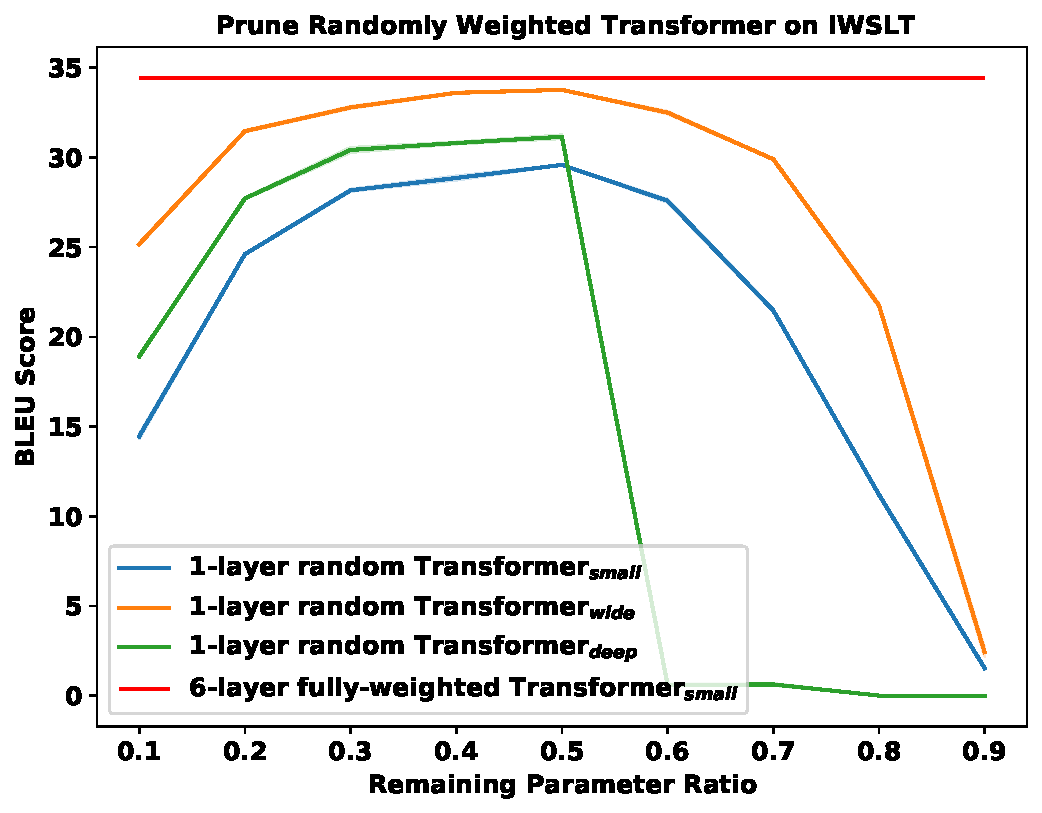
\includegraphics[width=0.8\linewidth]{fig/iwslt_widedeep.pdf}
        \vspace{-5pt}
    \caption{The effectiveness of depth and width.}
    \label{fig:res_iwslt_widedeep}
    \vspace{-10pt}
\end{figure}


\begin{figure}
    \centering
    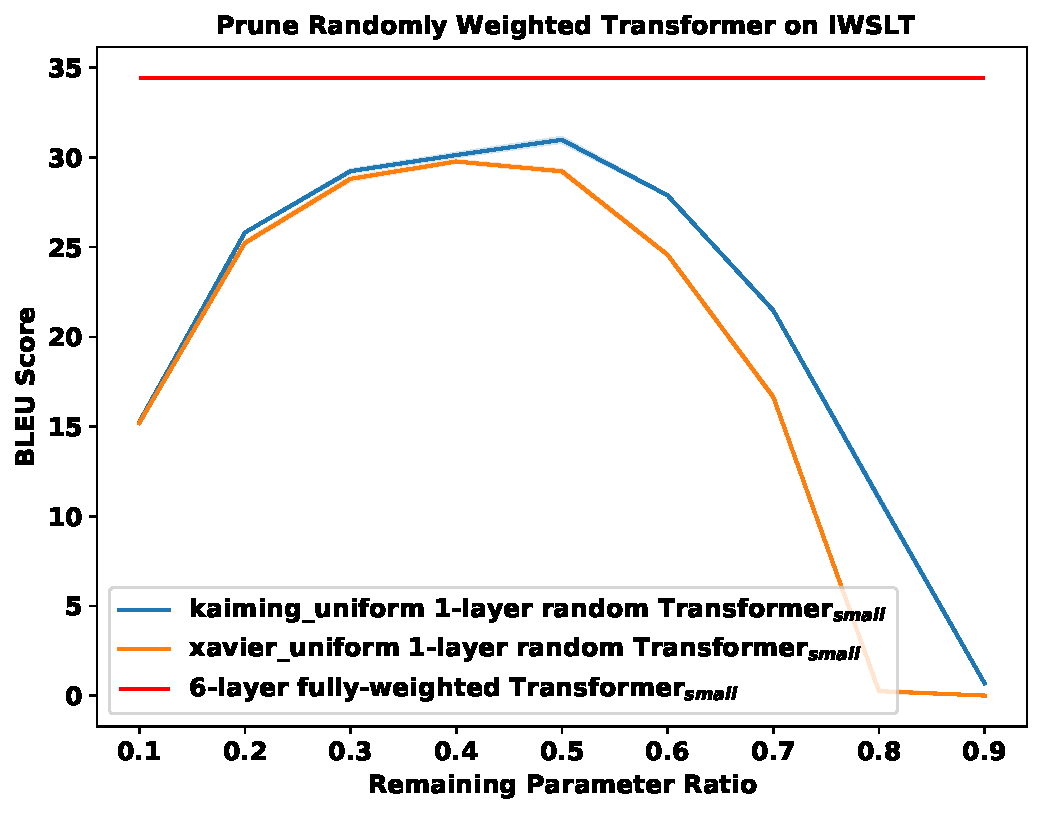
\includegraphics[width=0.8\linewidth]{fig/iwslt_init.pdf}
            \vspace{-5pt}
    \caption{The effectiveness of different initialization.}
    \label{fig:res_iwslt_init}
    \vspace{-10pt}
\end{figure}

\noindent\textbf{Different Initialization.}
Weight initialization is one of the critical components to the success of the random feature~\citep{Wieting:2019notraining,Ramanujan:2020hidden,shen2020reservoir}. 
We experiment with kaiming uniform~\citep{Ramanujan:2020hidden} and Xavier uniform~\citep{Vaswani:2017attention} initialization methods, and we scale the standard deviation by $\sqrt{1/\sigma}$ when we retain $\sigma$ randomized weights. 
As shown in~\fref{fig:res_iwslt_init}, the performance of the one-layer randomized Transformer decreases when we switch to the Xavier uniform. 
The degradation becomes larger when more randomized weights retain in the network. 





\begin{figure}
    \centering
    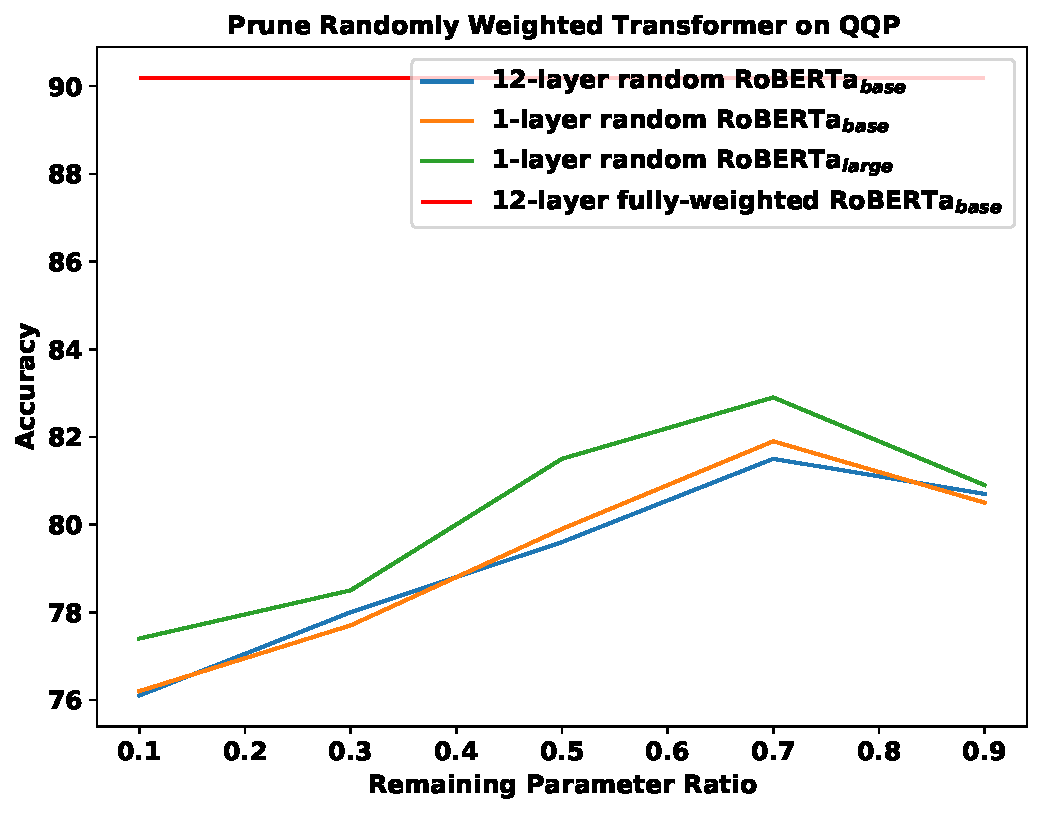
\includegraphics[width=0.8\linewidth]{fig/qqp.pdf}
    \caption{Prune Randomly Weighted Transformer performance on QQP .}
    \label{fig:qqp_base}
\end{figure}

\begin{figure}
    \centering
    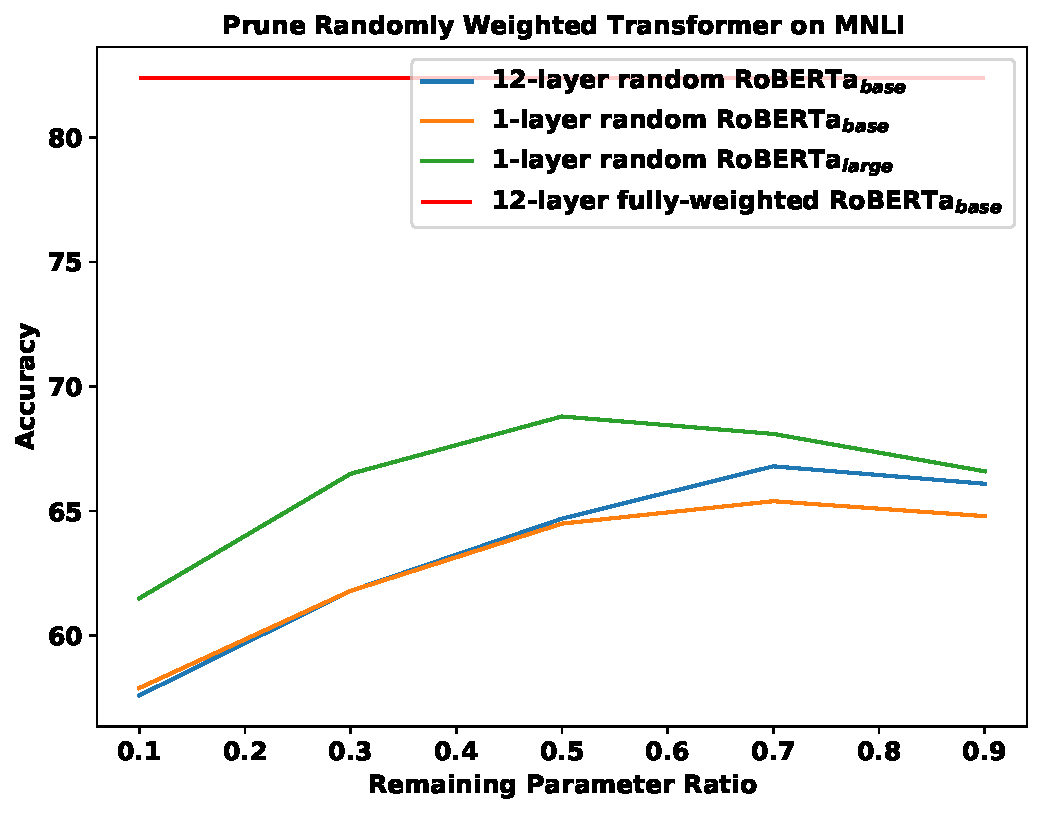
\includegraphics[width=0.8\linewidth]{fig/mnli.pdf}
    \caption{ Prune Randomly Weighted Transformer performance on MNLI.}
    \label{fig:mnli_base}
\end{figure}


\paragraph{QQP and MNLI results.} 
On QQP and MNLI, we experiment with RoBERTa$_\text{small}$ and RoBERTa$_\text{large}$, following \citet{Liu:2019roberta}. We use the pre-trained embedding layer of RoBERTa$_\text{base/large}$~\citep{Liu:2019roberta}. 
In~\fref{fig:qqp_base} and \ref{fig:mnli_base}, we show consistent results on QQP and MNLI, except that the best performing one-layer randomly weighted RoBERTa is achieved when we retain 70\% randomized weights, it reaches 79\%/91\% fully-weighted RoBERTa$_\text{base}$ accuracy on QQP and MNLI, respectively.  
The performance approaches 84\%/92\% of the aforementioned fully-weighted model performance when using the larger hidden size with one-layer randomly weighted RoBERTa$_\text{large}$. 

\paragraph{Implementation Details.} We evaluate on IWSLT14 de-en \citep{Cettolo:2015ReportOT} and WMT14 en-de \citep{bojar:2014-findings} for machine translation; QQP \citep{iyer2017qqp} and MultiNLI-matched (MNLI) \citep{Williams2017mnli} for natural language understanding.\footnote{For IWSLT, we follow the pre-processing steps in \citet{edunov:2018classical}. The train/val/test split is 129k/10k/6.8k sentences. 
For WMT, we follow pre-process as in \citet{Ott:2018scaling}, with 4.5M/16.5k/3k sentences in train/val/test.} 
We use 8 Volta V100 GPUs for WMT, and one V100 for IWSLT, QQP, and MNLI. The hyperparameters on IWSLT14 and WMT14 for training a one-layer randomized Transformer were set the same to the best-performing values from \citet{Ott:2018scaling} for training fully-weighted Transformer. The QQP and MNLI experiments followed \citet{Liu:2019roberta}. 







